%Part of/Parte di https://github.com/f-dinucci/appuntiMeccanicaFluidi/
%License/Licenza Creative Commons Attribution-ShareAlike 4.0 International (CC BY-SA 4.0) - attribution/attribuzione Francesco Di Nucci
%See also/Vedere anche https://creativecommons.org/licenses/by-sa/4.0/ and/e https://creativecommons.org/licenses/by-sa/4.0/legalcode
%
\section{Teorema di Kelvin}
\subsection{Teorema di Kelvin}
  %
	\begin{figure}[ht]
		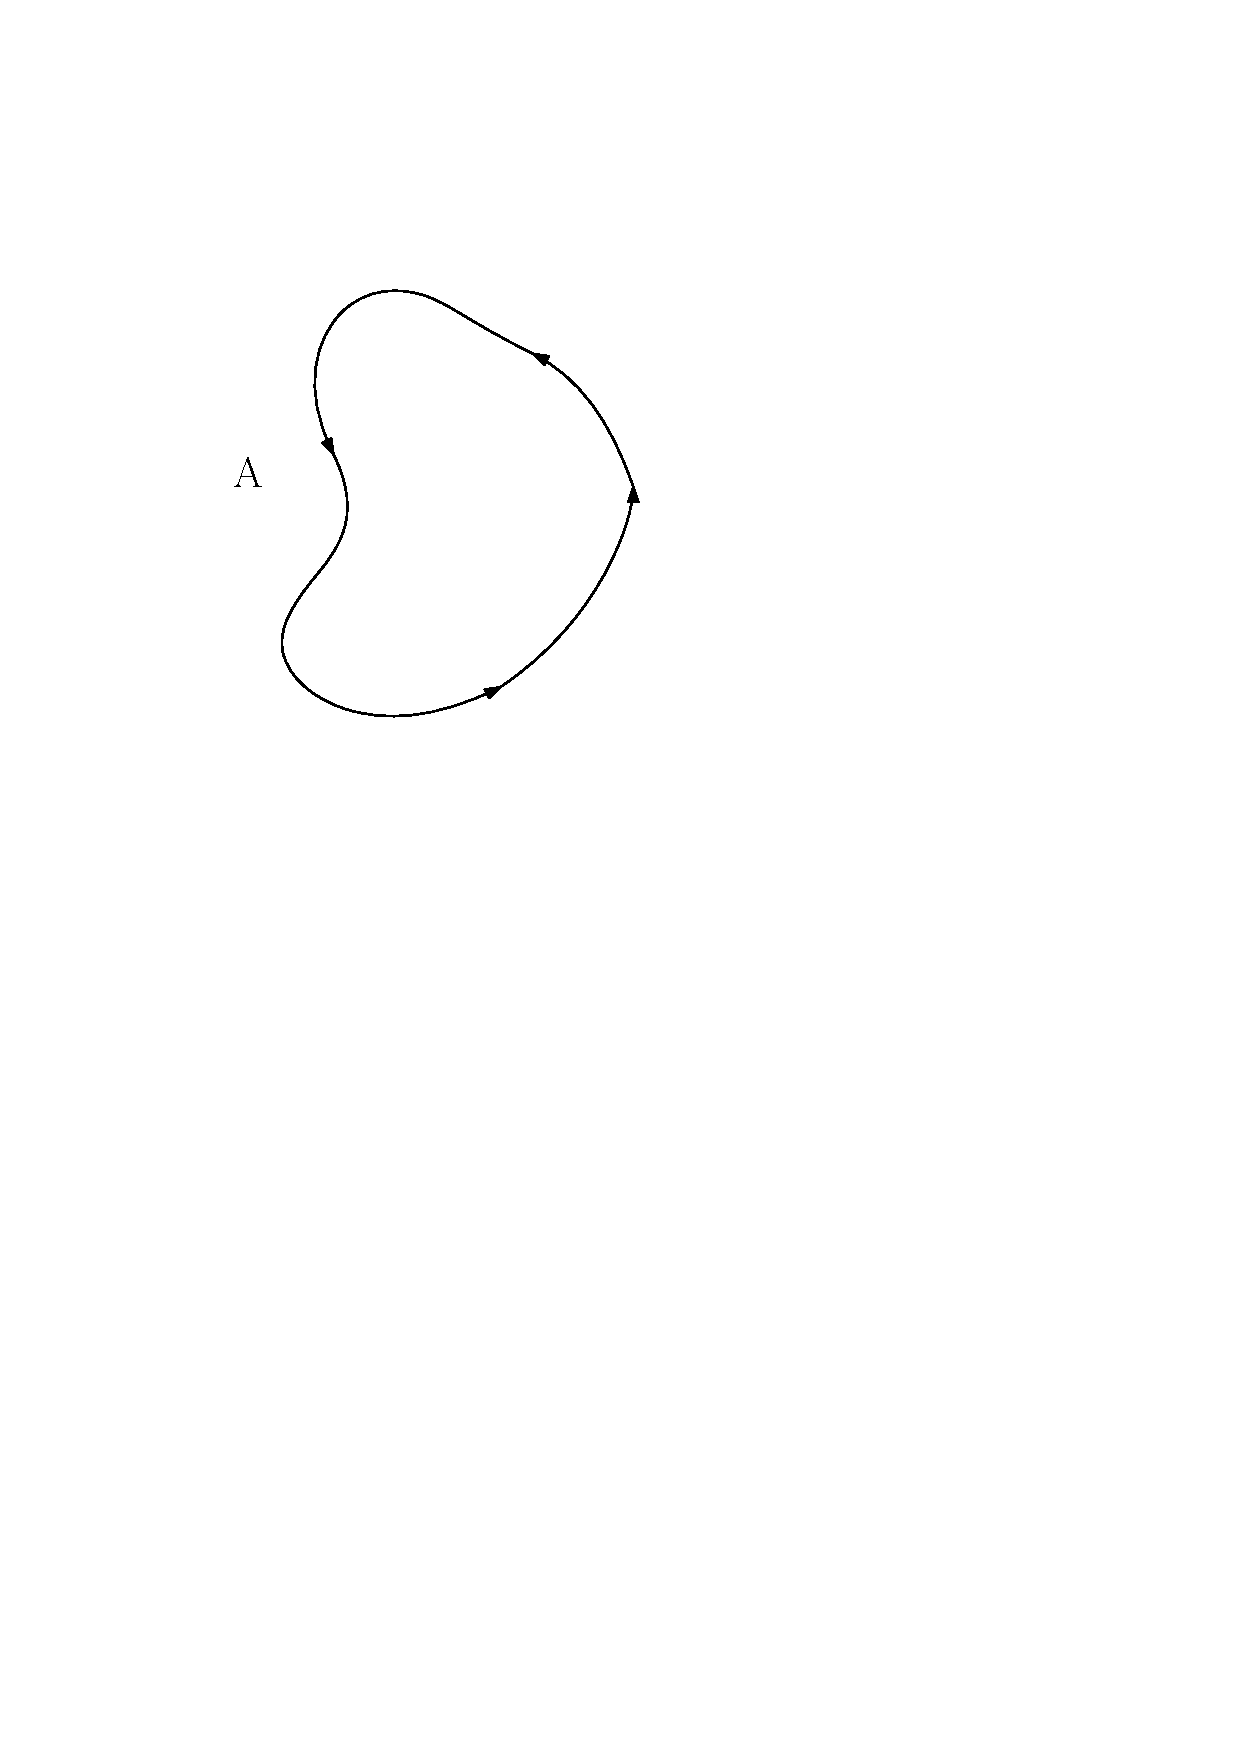
\includegraphics[scale=0.7]{./7.2 Teorema di Kelvin/7.2-1}
		\centering
		\caption{Linea nel fluido}
	\end{figure}
%
Il teorema di Kelvin riguarda la circolazione nel caso per il fluido valgano le equazioni di Eulero e si sia quindi in un caso irrotazionale.
La circolazione è l'integrale di linea di un vettore proiettato sul vettore tangente punto per punto alla linea.

Si può calcolare ad esempio per il vettore velocità lungo la linea $A$:
%
	\begin{equation*}
		\Gamma = \oint_A \uline{v} \vdot \uline{t} \dd{l} = \oint_A \uline{v} \vdot \dd{x}
	\end{equation*}
%
Per il teorema di Kelvin la circolazione è costante lungo una linea A trasportata con il fluido.

Si dimostra partendo dalla formula di Stokes (che è una formula matematica, valida in generale): 
%      
	\begin{equation*}
			\int \curl{\uline{v}} \uline{n} \dd{S} = \oint \uline{v} \vdot \uline{t} \dd{l}
	\end{equation*}
%			
Si applica all'equazione di Eulero e si vuole dimostrare che:	
%      
	\begin{equation*}
		\begin{gathered}
			\pdv{\uline{v}}{t} + \uline{v} \vdot \grad{\uline{v}} + \grad{p} = 0 
			\dv{\Gamma}{t} = \dv{t} \oint_{A(t)} \uline{v} \vdot \dd{\uline{x}} = 0\\
			\Gamma \text{ costante}
		\end{gathered}
	\end{equation*}
%

La linea A punto per punto ha la stessa velocità del fluido.
Si rappresenta la curva nello spazio in funzione dei parametri (tra cui il tempo) e si vede che la velocità di un punto della curva deve essere uguale a quella del fluido:
%
	\begin{equation*}
		\begin{gathered}
			A: x_i = x_i(S,t)\\
			\dv{x_i}{t} = v_i
		\end{gathered}
	\end{equation*}
%
Poi si torna all'integrale:
%
	\begin{equation*}
		\Gamma = \int v_i \pdv{x_i}{s} \dd{s}
	\end{equation*}
%
Derivando
%
	\begin{equation*}
		\begin{gathered}
			\dv{\Gamma}{t} = \oint \left( \frac{\mathrm{D} v_i}{\mathrm{D} t} \pdv{x_i}{s} + v_i \pdv{x_i}{s}{t} \right) \dd{s} =\\
			= \oint \left( - \pdv{p}{x_i} \pdv{x_i}{s} + v_i \pdv{v_i}{s} \right) \dd{s} = \\
			= \oint \left[ - \dv{p}{s} + \dv{s} \left( \frac{v^2}{2} \right) \right] = 0
		\end{gathered}
	\end{equation*}
%
L'integrale lungo il contorno chiuso della derivata di qualcosa è sempre nullo, dato che si otterrebbe la differenza tra punto iniziale e finale, ma i due punti coinciderebbero, quindi:			
%
	\begin{equation*}			
			\dv{\Gamma}{t} = 0
	\end{equation*}
%
Qualsiasi linea tracciata in una zona a vorticità nulla ha circuitazione nulla.
Le linee vengono trasportate con il fluido, quindi finché una regione a vorticità nulla è trasportata con il fluido, la sua vorticità rimane nulla, le zone di moto irrotazionale si mantengono trasportate con il fluido.

\subsection{Oggetto investito da fluido}
Un caso interessante è quello di un oggetto investito da un fluido (ad esempio un'automobile in moto, un aereo in volo etc.).
Ci si mette nel sistema di riferimento dell'oggetto, nel quale è il fluido a muoversi.
 %
	\begin{figure}[ht]
		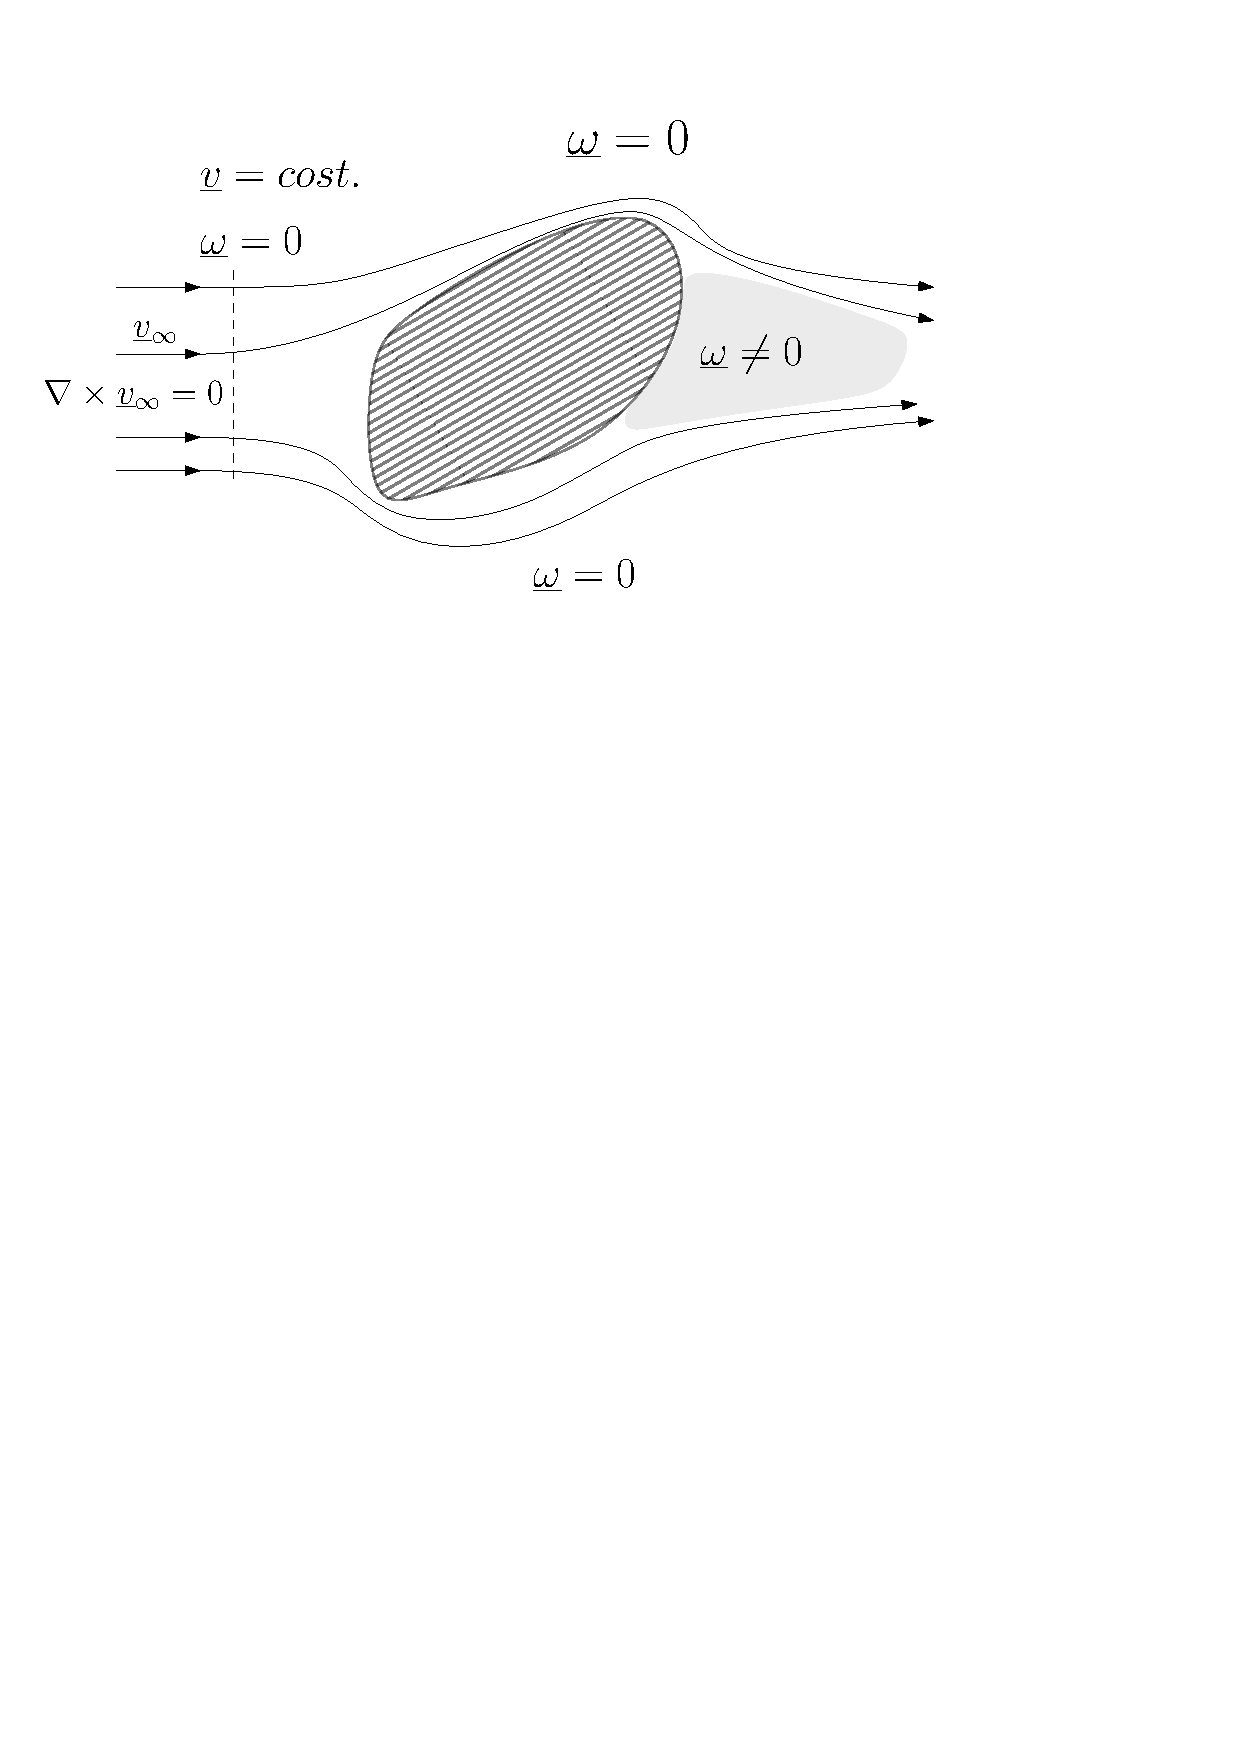
\includegraphics[scale=0.8]{./7.2 Teorema di Kelvin/7.2-2}
		\centering
		\caption{Oggetto investito da fluido}
	\end{figure}
%
La vorticità ad infinito è nulla, nei campi dove si può portare il fluido la vorticità rimane zero per il teorema di Kelvin.
Questo non vale nella zona dietro l'oggetto dove si ha la separazione del fluido e si forma una zona con vorticità non nulla, detta scia (è anche una zona di moto turbolento, questo si vedrà che ha conseguenze importanti sulla portanza e sulla resistenza).

\subsection*{Bibliografia 7.2}
\cite[Cap.\ 11.3]{CengelCimbala}\\
\cite[Cap.\ 10.2]{PnueliGutfinger}